
%%%%%%%%%%%%%%%%%%%%%%%%%%%%%%%%%%%%%%%%%%%%%%%%%%%%%%%%%%%%%%%%%%%%%%%%%%%%%%%%%%%%%%%%%%%%%%%%%%%%%%%%%%%%%%%


\begin{figure}[h!]

\begin{center}

    \caption{Receiver Operating Characteristic Curve} \label{fig:ROCcurve1}

        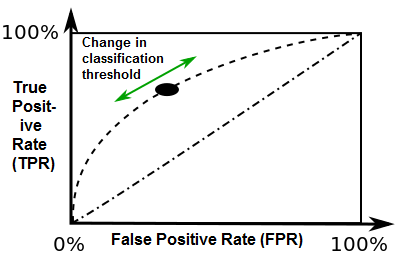
\includegraphics[scale=  0.75]{Figs/ROC/ROC_curve_3.png}



\end{center}

    \footnotesize

        \textbf{Receiver Operating Characteristic Curve:}
        True Positive Rate vs. False Positive Rate, for a particular value of the classification threshold.

% Terms in $KLD(\textcolor{blue}{f_1}, \textcolor{red}{f_2})
%  = \sum_{k = 1}^{K} \left\{ \textcolor{magenta}{\big( f_1(t_k) - f_2(t_k) \big)}
%         \textcolor{orange}{\log \left( \frac{f_1(t_k)}{f_2(t_k)} \right)} \right\}$

\end{figure}


%%%%%%%%%%%%%%%%%%%%%%%%%%%%%%%%%%%%%%%%%%%%%%%%%%%%%%%%%%%%%%%%%%%%%%%%%%%%%%%%%%%%%%%%%%%%%%%%%%%%%%%%%%%%%%%

